\section{Ablation studies: details}\label{si:ablations}

This section gives the full protocol and discussion of the ablation studies summarised in Section~\Mref{sec:ablations}. Tables for the stratifier (A1) and for small-sample inference (A4) are in the main text (Tables~\Mref{tab:abl-design} and~\Mref{tab:abl-inference}); the others are below.

This section varies one ingredient of PATTERN-DIF at a time and asks two questions: does the estimator remain valid, and how much efficiency is gained or lost relative to the default? The default is the method of the main study: strata $(G_i,K_i)$ with strata smaller than 50 merged within group, weighted generalised Neyman allocation \citep{neyman1934} computed with the ensemble-mean proxy $\pi_i$, a floor of 10 labels per stratum, the stratified difference estimator with $\lambda=1$ and the same proxy, and 95\% Wald intervals from the linearisation variance. The estimator that uses the proxy only to allocate labels, the plain (Horvitz--Thompson) estimator, is called HT or $\lambda=0$. Because the proxy now enters the estimator as well as the allocation, the proxy ablations report the two roles separately, and every ablation reports the difference estimator and, where it is informative, HT on the same samples. All results come from \texttt{experiments/label\_ablations\_dif.py} (helpers in \texttt{tcs/labeling\_variants\_dif.py}) and are stored in \texttt{results/label\_ablations\_dif.json}. An earlier version of this study, in which the plain estimator was the default, is not reported; where its conclusions differ they are noted below.

\paragraph{Protocol.} We use the eleven cached pools and budgets $L\in\{250,500,1000\}$ with $L\le N/4$ (29 setting--budget cells) and $R=150$ replications per cell and design. The first seven designs (SRS, GROUP, PATTERN and four alternative stratifiers) draw the same samples as an earlier version of this ablation study that used the plain estimator throughout (\texttt{results/label\_ablations.json} in the repository); we call it the earlier plug-in study and refer to its numbers where they are compared, so that differences between the two studies are due to the estimator alone. There are 108 comparison targets for the 36 pairs of nine models; targets whose numerator vanishes identically in the pool are exact for every design and are excluded (only Law school, where 57 remain). Efficiency is the per-target ratio $\mathrm{MSE}_{\mathrm{SRS}}/\mathrm{MSE}_{\mathrm{design}}$ with SRS and the plain estimator as reference, clipped to $[10^{-4},10^{4}]$, summarised by the median over targets and then over cells. ``Rel.'' is the median over cells of $\mathrm{MSE}_{\mathrm{PATTERN\text{-}DIF}}/\mathrm{MSE}_{\mathrm{variant}}$ (above one favours the variant) and ``Win'' the share of cells with Rel.\ above one. Coverage is the mean over targets and the worst target. With $R=150$ the Monte Carlo standard error of one coverage is about 0.018 and the minimum over 108 targets that all cover exactly 95\% has mean 0.90, so worst-target coverage near 0.90 is consistent with nominal behaviour and values well below 0.88 are not. A design with more strata than the budget can feed at 10 labels each uses the floor $\max(2,\lfloor 0.8L/H\rfloor)$. Undefined estimates occurred in at most 0.7\% of replications.

\subsection{Stratifier (A1)}

Table~\Mref{tab:abl-design} varies the stratifier; per-cell values are in Table~\ref{tab:abl-app-eff-design} of Section~\ref{si:ablation-tables}. On the same samples the difference estimator is more efficient than HT in all 29 cells (median ratio 1.67, range 1.36 to 14.5 in Law school), and its efficiency against SRS is 6.3 at every budget, compared with 3.6 to 4.3 for HT. The two gains are not additive: SRS with the difference estimator (SRS-DIF, i.e.\ PPI of \citealt{angelopoulos2023ppi} with the ensemble proxy) gains a factor 1.9, the PATTERN design with HT a factor 4.0 over all budgets, and the product of these medians (7.5) exceeds the combined gain.

The stratifier conclusions of the earlier study carry over. Group $\times$ agree/disagree keeps 74\% of the default's precision (earlier 71\%) and the joint pattern of the three models agreeing most with the ensemble keeps 38\% (earlier 37\%): the count $K_i$ is what matters, and three models cannot isolate the disagreement among 36 pairs. Splitting each $(G,K)$ cell at the median of $\pi_i$ is a tie (Rel.\ 1.01, better in 15 of 29 cells; by budget 0.99, 0.97, 1.04), as are tertile bins (0.99), whose extra strata eat the budget through the floor (3 to 9 labels where it binds). We keep $K_i$. The allocation tailored to the variance of the difference estimator (\texttt{'resid'} in \texttt{tcs.labeling\_dif}) is not better than the plain allocation (Rel.\ 0.96, better in 13 cells). The references that drop an ingredient lose clearly: GROUP-DIF and SRS-DIF keep 28\%, proportional allocation 57\% (earlier 52\%) and the gap-targeted allocation of A5 74\% (earlier 74\%). Coverage hardly depends on the stratifier (mean 0.938 to 0.946).

\subsection{Proxy and the role of $\lambda$ (A2)}

The proxy now has two jobs, and the ablation separates them (Table~\ref{tab:abl-proxy}; Figure~\ref{fig:abl-proxy} in Section~\ref{si:ablation-tables} shows the per-cell spread). The first block uses a proxy $\tilde\pi$ only to allocate labels and analyses the sample with HT. The second uses the same $\tilde\pi$ in the allocation and in the estimator, through the proxy mean $\psi_i=\tilde\pi_iu_i+(1-\tilde\pi_i)v_i$. The third allocates with $\tilde\pi$ but keeps the ensemble proxy in the estimator.

\emph{Allocation only.} As in the earlier study, the allocation is insensitive to the proxy. With HT, every proxy gives a median efficiency of 3.95 to 4.05 against 3.97 for the ensemble mean, including the reversed proxy $1-\pi$, the shuffled proxy and the constant 0.5; allocation by the true labels gives 3.71. With the ensemble proxy kept in the estimator, the alternative allocations keep 99\% to 101\% of the default's precision (Rel.\ in Table~\ref{tab:abl-proxy}, last block), with per-cell ratios between 0.86 and 1.4 except in Churn at $L=500$, where the constant, naive Bayes and shuffled proxies label the small disagreement strata exhaustively and gain factors of 19, 13 and 6 (1.8 for the logistic proxy). The reason is the same as before: the influence values vary within a stratum mainly through the differences $\hat y_{mi}-\hat y_{ji}$, known without labels. What matters in the allocation is that it is Neyman-type rather than proportional (Rel.\ 0.57).

\emph{Proxy in the estimator.} Here the proxy matters. Replacing the ensemble mean by a single model costs 13\% (logistic regression) or 42\% (naive Bayes, whose probabilities are extreme); the constant 0.5 costs 16\%, a shuffled proxy 47\%, a noisy proxy 39\% and the reversed proxy 34\% (Table~\ref{tab:abl-proxy}, middle block). The difference estimator remains unbiased and its coverage is unaffected (mean 0.940 to 0.949), as the theory predicts, so a poor proxy costs efficiency only. A corrupted proxy also removes the gain over HT on the same sample: the median ratio of DIF to HT is 0.96 for the shuffled and noisy proxies and 1.00 for naive Bayes, against 1.67 for the ensemble, and DIF is less efficient than HT in 19, 18 and 15 of 29 cells for these three. The constant keeps most of the gain (ratio 1.40) because $\psi_i$ still carries the known structure of $u_i,v_i$.

\begin{table}[t]
\centering\footnotesize
\setlength{\tabcolsep}{4pt}
\caption{Proxy ablation (A2). Eff.: median over all 29 cells of the median-over-targets efficiency vs SRS (plain estimator); Rel.: relative to PATTERN-DIF with the ensemble proxy (as in Table~\Mref{tab:abl-design}); worst: mean over cells of the worst-target coverage; mean: mean coverage. In the first block the proxy enters only the allocation and the sample is analysed with HT; in the second it enters allocation and estimator; in the third only the allocation, the estimator keeps the ensemble proxy. The true-label proxy is not defined as an estimator proxy (the estimator would be exact).}
\label{tab:abl-proxy}
\resizebox{\textwidth}{!}{\begin{tabular}{lcccccccccc}
\toprule
 & \multicolumn{3}{c}{Proxy in allocation only (HT)} & \multicolumn{4}{c}{Proxy in both (DIF)} & \multicolumn{2}{c}{DIF, ensemble in estimator} \\
\cmidrule(lr){2-4}\cmidrule(lr){5-8}\cmidrule(lr){9-10}
Proxy & Eff. & Rel. & worst & Eff. & Rel. & mean & worst & Eff. & Rel. \\
\midrule
Ensemble mean $\pi$ (default) & 3.97 & 0.65 & 0.858 & 6.27 & 1.00 & 0.945 & 0.877 & 6.27 & 1.00 \\
Single model (logistic) & 3.96 & 0.64 & 0.861 & 5.56 & 0.87 & 0.943 & 0.886 & 6.01 & 0.99 \\
Single model (naive Bayes) & 4.05 & 0.63 & 0.858 & 3.88 & 0.58 & 0.942 & 0.873 & 5.99 & 1.01 \\
Constant 0.5 & 3.97 & 0.62 & 0.850 & 5.71 & 0.84 & 0.940 & 0.858 & 6.01 & 0.99 \\
$\pi$ shuffled within group & 3.95 & 0.62 & 0.854 & 3.70 & 0.53 & 0.949 & 0.889 & 6.12 & 0.99 \\
$\pi$ with logit noise (sd 2) & 4.05 & 0.64 & 0.854 & 3.46 & 0.61 & 0.949 & 0.877 & 5.91 & 0.99 \\
Reversed, $1-\pi$ & 3.99 & 0.63 & 0.859 & 4.38 & 0.66 & 0.941 & 0.872 & 6.23 & 0.99 \\
True labels (allocation only) & 3.71 & 0.64 & 0.865 & -- & -- & -- & -- & 6.01 & 1.00 \\
\addlinespace
Proportional allocation (no proxy in allocation) & 2.05 & 0.38 & 0.819 & 3.75 & 0.57 & 0.943 & 0.877 & -- & -- \\
\bottomrule
\end{tabular}
}
\end{table}

\emph{The weight $\lambda$.} Table~\ref{tab:abl-lambda} (Section~\ref{si:ablation-tables}) compares $\lambda=0$ (HT), $\lambda=1$ (default) and a $\lambda$ tuned per stratum and target on the labelled units and clipped to $[0,1]$ \citep[as in PPI++ and StratPPI;][]{angelopoulos2026ppipp,fisch2024stratppi}. With the ensemble proxy the tuned version is slightly more efficient than $\lambda=1$ (median Rel.\ 1.016, better in 24 of 29 cells; 1.026 at $L=250$) but it undercovers: mean 0.923, worst target 0.799 on average and 0.227 in Law school at $L=250$, against 0.945, 0.877 and 0.633 for $\lambda=1$. The tuned weights are estimated from a few labels per stratum and the variance estimate ignores that. With a degraded proxy the tuned version is the more efficient of the three (shuffled 5.2, noisy 5.1, reversed 5.4, against 3.7, 3.5 and 4.4 at $\lambda=1$ and about 4.0 for HT), because it shrinks the correction, but again at coverage 0.92 to 0.93. Neither alternative is better than $\lambda=1$ with the ensemble proxy in both efficiency and validity, so we keep $\lambda=1$. Tuning is worth considering only when the proxy is known to be poor and some undercoverage is acceptable.

\subsection{Number of compared models (A3)}

For $M\in\{2,3,5\}$ we drew three random subsets of the nine models per size (the subsets of the earlier study), rebuilt strata, proxy and estimands from the subset only, and compared PATTERN-DIF and PATTERN-HT with SRS on the $3\binom{M}{2}$ targets. Subsets in which all models agree on every instance are dropped. Table~\ref{tab:abl-models} and Figure~\ref{fig:abl-models} show, as before, that the gain is governed by the share of the pool on which the compared models disagree rather than by $M$: the Spearman correlation between log efficiency and the disagreement share across the 284 configurations is $-0.72$, $-0.74$ and $-0.76$ at $L=250$, 500 and 1000 (HT: $-0.81$, $-0.78$, $-0.79$), and within settings at $L=250$ it is negative in all eleven (median $-0.43$). At $L=250$ the median efficiency of PATTERN-DIF is 17.2 when the compared models disagree on less than 10\% of the pool, 12.5 for 10 to 20\%, 4.8 for 20 to 40\% and 3.8 above 40\%. What the difference estimator changes is the size of the gain over HT, which grows with $M$ from 1.15 at $M=2$ to 1.67 at $M=9$. The log ratio of DIF to HT is positively correlated with the disagreement share (0.09, 0.19, 0.34 by budget). The correction therefore helps most where the design alone helps least, but it does not remove the dependence on disagreement. Coverage is not affected by $M$ (mean 0.945 to 0.950); the worst-target figures cannot be compared across rows, because the number of targets grows from 3 to 108.

\begin{table}[t]
\centering\small
\caption{Number of compared models (A3). Configs: (setting, budget, subset) combinations; Disagr.: median share of the pool on which not all $M$ models agree. Efficiency: median over configurations of the median-over-targets $\mathrm{MSE}_{\mathrm{SRS}}/\mathrm{MSE}$. DIF/HT: median ratio of the two efficiencies on the same sample. Coverage: PATTERN-DIF, Wald.}
\label{tab:abl-models}
\resizebox{\textwidth}{!}{\begin{tabular}{rccccccccc}
\toprule
 & & & \multicolumn{3}{c}{PATTERN-DIF vs SRS} & \multicolumn{1}{c}{PATTERN-HT vs SRS} & & \multicolumn{2}{c}{Coverage (DIF)} \\
\cmidrule(lr){4-6}\cmidrule(lr){9-10}
$M$ & Configs & Disagr. & $L=250$ & 500 & 1000 & all $L$ & DIF/HT & mean & worst \\
\midrule
2 & 87 & 0.133 & 9.48 & 12.58 & 9.28 & 8.37 & 1.15 & 0.950 & 0.933 \\
3 & 84 & 0.193 & 8.29 & 10.70 & 8.57 & 6.44 & 1.27 & 0.949 & 0.919 \\
5 & 84 & 0.294 & 7.62 & 6.64 & 7.08 & 4.78 & 1.52 & 0.946 & 0.904 \\
9 & 29 & 0.396 & 6.27 & 6.18 & 6.37 & 3.97 & 1.67 & 0.945 & 0.877 \\
\bottomrule
\end{tabular}
}
\end{table}

\begin{figure}[t]
\centering
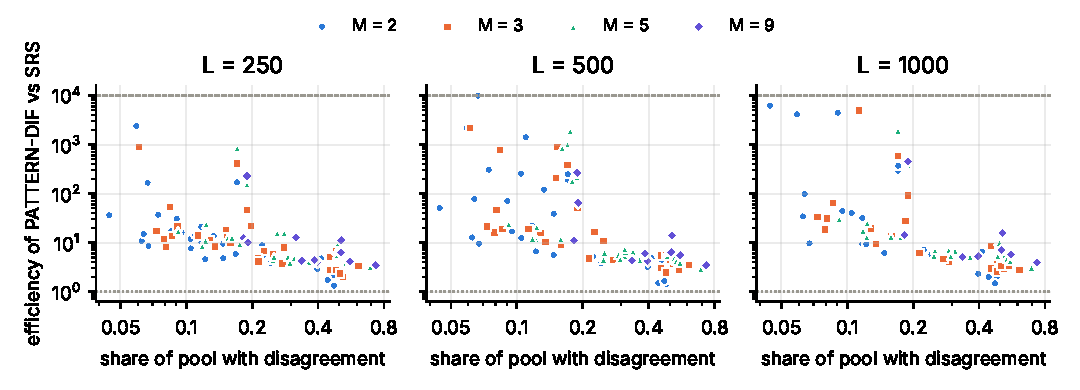
\includegraphics[width=\textwidth]{figures/abl_dif_models_disagreement.pdf}
\caption{Efficiency of PATTERN-DIF relative to SRS (median over targets) against the share of the pool on which the compared models do not all agree, for random subsets of $M$ models in every setting (A3). Both axes are logarithmic; the dotted line marks parity and the dashed line the clipping value $10^4$.}
\label{fig:abl-models}
\end{figure}

\subsection{Small-sample inference (A4)}

With the plain estimator the main study found worst-target coverage near 0.5 at $L=250$ in Churn and Law school, traced to strata whose sampled units show no variation in the influence values. The difference estimator removes most of this: the residual $\xi_i=t_i-\psi_i=(Y_i-\pi_i)(u_i-v_i)$ varies even when no positive is sampled, no (replication, target) pair had a standard error of exactly zero (plain estimator: up to 1.0\% in Law school), and the worst-target Wald coverage in Churn at $L=250$ rises from 0.47 to 0.91 (Table~\Mref{tab:abl-inference}, Figure~\ref{fig:abl-coverage}). The shortfalls that remain are of a different kind. Over the 29 cells the worst-target Wald coverage is below 0.85 in five cells (Law school 0.63, MAGIC 0.78 and Adult-sex 0.82 at $L=250$, Bank 0.83 and Phoneme 0.83 at $L=500$), against five cells for HT and six for SRS-DIF. The worst target is a TPR contrast in 17 of 29 cells (FPR in 4, error difference in 8). On average over cells its mean standard error is 0.90 of the Monte Carlo standard deviation (0.99 for the median target) and its bias is below 0.16 standard deviations, so the intervals are too short rather than off-centre, which is consistent with a linearisation error in a ratio with few sampled positives in the smaller group (we did not test this further).

None of the standard corrections closes this gap. A $t$ quantile with \citet{satterthwaite1946} degrees of freedom adds 1\% to the width and moves the mean worst target at $L=250$ from 0.852 to 0.865. The stratified bootstrap percentile interval \citep{efron1979}, which resamples labelled residuals within strata ($B=999$, no finite-population correction; \citealt{raowu1988} discuss a rescaled version), is 11\% wider and a little conservative (mean coverage 0.961 over all cells), with worst target 0.878 and minimum 0.767. The proxy variance floor of \texttt{tcs.labeling\_dif} replaces the sample variance of a stratum by its proxy residual variance when the former is exactly zero ('zero') or by the larger of the two in every stratum ('max'). The 'zero' floor leaves the width unchanged (1.002) and lifts the minimum over cells from 0.633 to 0.780, entirely through Law school (0.90 at $L=250$); combined with the $t$ quantile the mean worst target is 0.885 and four cells stay below 0.85. Only the 'max' floor reaches 0.92 in every cell (mean worst target 0.948), and it is conservative: mean coverage 0.985 at $L=250$, width 1.67 times Wald on average, 1.25 in the median and 4.9 in Law school. For SRS-DIF Wald coverage is poor (minimum 0.27) and the bootstrap worse (0.10); 'max' repairs it (minimum 0.88) at 23\% extra width. The floors were designed after seeing the failure of the plain estimator on these pools, so the 'zero' result for Law school is in-sample (the residual floor is discussed further in Section~\ref{sec:simulation}). An independent check on synthetic pools (\texttt{results/floor\_check.json}) found that the floor leaves the interval width unchanged (median ratio 1.00).

\begin{figure}[t]
\centering
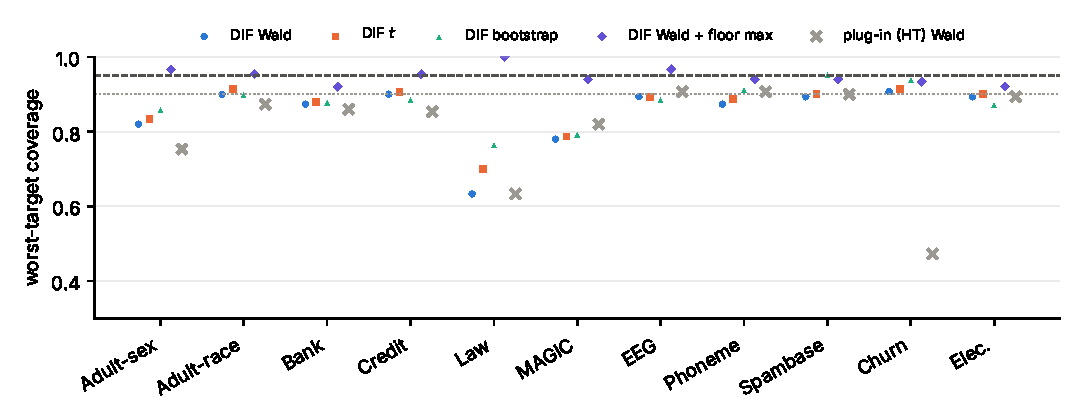
\includegraphics[width=\textwidth]{figures/abl_dif_coverage_L250.pdf}
\caption{Worst-target coverage at $L=250$ in each setting for PATTERN-DIF under four interval methods and for the plain estimator (A4). Dashed line: nominal 0.95; dotted line: expected minimum over 108 targets of 150-replicate coverage if every target covered exactly 95\% (0.90; Law school has 57 targets).}
\label{fig:abl-coverage}
\end{figure}

\subsection{Ranking models by the equalised-odds gap (A5)}

Practitioners also look at each model's equalised-odds gap $EO_m=\max(|\Delta^{TPR}_m|,|\Delta^{FPR}_m|)$ \citep{hardt2016} and rank models by it. We computed the plug-in $\widehat{EO}_m=f_{EO}(\hat T)$ from the totals of the same samples, with the difference estimator (DIF totals) and the plain estimator, and recorded the RMSE, the probability $P$ that the model with the smallest estimated gap has the smallest true gap, Kendall's $\tau$ \citep{kendall1938} between estimated and true gaps, and the bias. We also include a variant of PATTERN whose allocation targets the $2M$ per-model gaps instead of the comparison contrasts (gap-targeted). Table~\ref{tab:abl-eo} summarises the results; per-cell values are in Table~\ref{tab:abl-app-eo}.

The plug-in $\widehat{EO}_m$ is biased upwards, as a maximum of absolute values must be (mean bias 0.042 for SRS, 0.026 for PATTERN with HT, 0.024 for PATTERN-DIF, 0.019 for the gap-targeted variant with DIF). PATTERN-DIF is more accurate than SRS in the median (efficiency 1.94 to 2.21) and identifies the best model more often (mean $P$ 0.50 against 0.35 at $L=250$; 0.46 against 0.21 without Law school, where six models tie, and EEG, where the best model leads by 0.039). PATTERN with HT reaches efficiency 1.80 to 1.94 and $P$ 0.46 to 0.62, so the difference estimator adds little for this purpose. The gain is not uniform: PATTERN-DIF is less accurate than SRS in all Electricity cells (0.57 to 0.73) and in MAGIC at $L=1000$, because the allocation spends labels on disagreement whereas the gap of one model depends on all of its positive predictions. SRS-DIF has about the same RMSE efficiency (2.08 to 2.28) but a lower $P$ (0.42 at $L=250$) and $\tau$ (0.41). The gap-targeted allocation with the difference estimator is the best design here (efficiency 2.30 to 2.61, $P=0.49$, 0.56, 0.65 and $\tau=0.48$, 0.54, 0.64 by budget; never worse than SRS except in Law school) but it keeps only 74\% of the precision for the comparison contrasts (Table~\Mref{tab:abl-design}). In Law school the models are near-perfect and six have $EO_m=0$ exactly; the plain estimator then returns exactly zero for them and wins every tie, whereas the difference estimator does not (MSE ratio clipped at $10^{-4}$). When the true margin to the next model is 0.002 or less (Adult-sex, Bank, Credit card default, Churn) identification is hard for every design: $P$ for PATTERN-DIF is at most 0.55 at the largest budget and 0.11 in Credit card default (margin 0.0003).

\begin{table}[t]
\centering\footnotesize
\setlength{\tabcolsep}{4pt}
\caption{Equalised-odds gap (A5). Eff.: median over cells of the median over models of $\mathrm{MSE}_{\mathrm{SRS}}/\mathrm{MSE}$ for $\widehat{EO}_m$ (cells in which both are exactly zero are skipped); $P$: mean probability that the estimated smallest-gap model has the smallest true gap; $\tau$: mean Kendall $\tau$ between estimated and true $EO_m$. DIF: totals from the difference estimator; plug-in: plain estimator.}
\label{tab:abl-eo}
\begin{tabular}{lccccccccc}
\toprule
 & \multicolumn{3}{c}{$L=250$} & \multicolumn{3}{c}{$L=500$} & \multicolumn{3}{c}{$L=1000$} \\
\cmidrule(lr){2-4}\cmidrule(lr){5-7}\cmidrule(lr){8-10}
Design & Eff. & $P$ & $\tau$ & Eff. & $P$ & $\tau$ & Eff. & $P$ & $\tau$ \\
\midrule
SRS (plug-in) & 1.00 & 0.35 & 0.32 & 1.00 & 0.42 & 0.39 & 1.00 & 0.49 & 0.48 \\
SRS-DIF (PPI) & 2.08 & 0.42 & 0.41 & 2.22 & 0.47 & 0.45 & 2.28 & 0.53 & 0.55 \\
GROUP, plug-in & 1.07 & 0.37 & 0.34 & 1.10 & 0.43 & 0.42 & 1.63 & 0.51 & 0.52 \\
PATTERN, plug-in (HT) & 1.83 & 0.46 & 0.45 & 1.80 & 0.51 & 0.49 & 1.94 & 0.62 & 0.62 \\
PATTERN-DIF (default) & 1.94 & 0.50 & 0.48 & 1.94 & 0.53 & 0.51 & 2.21 & 0.61 & 0.62 \\
Gap-targeted, plug-in & 2.03 & 0.44 & 0.43 & 2.29 & 0.52 & 0.51 & 2.54 & 0.59 & 0.61 \\
Gap-targeted, DIF & 2.30 & 0.49 & 0.48 & 2.61 & 0.56 & 0.54 & 2.51 & 0.65 & 0.64 \\
ORACLE-ALLOC, DIF & 2.02 & 0.50 & 0.47 & 1.77 & 0.54 & 0.52 & 1.93 & 0.57 & 0.60 \\
\bottomrule
\end{tabular}

\end{table}

\paragraph{Summary.} With the difference estimator the ablation conclusions about the design are those of the earlier plug-in study: the count $K_i$ is the stratifier worth having, Neyman rather than proportional allocation matters, the allocation is insensitive to the proxy, and the gain depends on how often the compared models disagree. Three things differ. First, the proxy now matters in the estimator, where a poor proxy costs up to half of the efficiency and removes the advantage over HT, although coverage is unaffected; the ensemble mean was never beaten there. Second, the difference estimator removes the zero-variance failure of the plain estimator, so the proxy variance floor has become a cheap safeguard ('zero', no loss of width) rather than a 19\% widening, and the remaining undercoverage of rate contrasts at $L=250$ is not fixed by $t$ quantiles, the bootstrap or the floor; only the conservative 'max' floor reaches nominal worst-target coverage. Third, for ranking models by $EO_m$ itself the gap-targeted allocation with the difference estimator is better than the default. Neither tuned $\lambda$ nor proxy-bin strata beat the default consistently, and we keep it; we recommend reporting the Wald interval with the 'zero' floor, which costs nothing in width.
